% (find-LATEX "2021-2-C3-diag-nums.tex")
% (defun c () (interactive) (find-LATEXsh "lualatex -record 2021-2-C3-diag-nums.tex" :end))
% (defun C () (interactive) (find-LATEXsh "lualatex 2021-2-C3-diag-nums.tex" "Success!!!"))
% (defun D () (interactive) (find-pdf-page      "~/LATEX/2021-2-C3-diag-nums.pdf"))
% (defun d () (interactive) (find-pdftools-page "~/LATEX/2021-2-C3-diag-nums.pdf"))
% (defun e () (interactive) (find-LATEX "2021-2-C3-diag-nums.tex"))
% (defun l () (interactive) (find-LATEX "2021-2-C3-diag-nums.lua"))
% (defun o () (interactive) (find-LATEX "2021-1-C3-curvas-de-nivel.tex"))
% (defun u () (interactive) (find-latex-upload-links "2021-2-C3-diag-nums"))
% (defun v () (interactive) (find-2a '(e) '(d)))
% (defun d0 () (interactive) (find-ebuffer "2021-2-C3-diag-nums.pdf"))
% (defun cv () (interactive) (C) (ee-kill-this-buffer) (v) (g))
%          (code-eec-LATEX "2021-2-C3-diag-nums")
% (find-pdf-page   "~/LATEX/2021-2-C3-diag-nums.pdf")
% (find-sh0 "cp -v  ~/LATEX/2021-2-C3-diag-nums.pdf /tmp/")
% (find-sh0 "cp -v  ~/LATEX/2021-2-C3-diag-nums.pdf /tmp/pen/")
%     (find-xournalpp "/tmp/2021-2-C3-diag-nums.pdf")
%   file:///home/edrx/LATEX/2021-2-C3-diag-nums.pdf
%               file:///tmp/2021-2-C3-diag-nums.pdf
%           file:///tmp/pen/2021-2-C3-diag-nums.pdf
% http://angg.twu.net/LATEX/2021-2-C3-diag-nums.pdf
% (find-LATEX "2019.mk")
% (find-CN-aula-links "2021-2-C3-diag-nums" "3" "c3m212dn" "c3dn")

% «.videos»		(to "videos")
% «.video-diagonal»	(to "video-diagonal")
% «.videos-antigos»	(to "videos-antigos")
%
% «.defs»		(to "defs")
% «.title»		(to "title")
% «.minecraft»		(to "minecraft")
% «.postes»		(to "postes")
% «.eq-da-superficie»	(to "eq-da-superficie")
% «.figuras-3D»		(to "figuras-3D")
% «.exercicios-12»	(to "exercicios-12")
% «.exercicio-1»	(to "exercicio-1")
% «.exercicio-2»	(to "exercicio-2")
% «.exercicio-2-maxima»	(to "exercicio-2-maxima")
% «.exercicio-4»	(to "exercicio-4")
% «.exercicio-5»	(to "exercicio-5")
%   «.diag-sinais-em-R»	(to "diag-sinais-em-R")
% «.exercicio-6»	(to "exercicio-6")
% «.exercicio-7»	(to "exercicio-7")
% «.signif-geom-ztt»	(to "signif-geom-ztt")
% «.exercicio-8»	(to "exercicio-8")
% «.cabos-na-diagonal»	(to "cabos-na-diagonal")
% «.sups-quadrs»	(to "sups-quadrs")
% «.exercicio-4»	(to "exercicio-4")
%
% «.PDFs-antigos»	(to "PDFs-antigos")
% «.links»		(to "links")
%
% «.djvuize»		(to "djvuize")



% «videos»  (to ".videos")

% «video-diagonal»  (to ".video-diagonal")
% (c3m212dna            "video-diagonal")
% (find-ssr-links     "c3cd" "2021-2-c3-cabos-na-diagonal" "nxsIK0tPWAI")
% (code-eevvideo      "c3cd" "2021-2-c3-cabos-na-diagonal" "nxsIK0tPWAI")
% (code-eevlinksvideo "c3cd" "2021-2-c3-cabos-na-diagonal" "nxsIK0tPWAI")
% (find-yttranscript-links "c3cd" "nxsIK0tPWAI")
% (find-c3cdvideo "0:00")
% (find-c3cdvideo "04:38" "a gente não sabe direito o que que tem no")
% (find-c3cdvideo "04:39"   "miolo desse quadrado e tem duas coisas naturais")
% (find-c3cdvideo "06:58" "se a gente vê começa a mudar o ângulo dessa")
% (find-c3cdvideo "07:01"   "curva pra gente ver ela desse jeito")
% (find-c3cdvideo "13:10" "uma parte do quadrado tá horizontal e a")
% (find-c3cdvideo "13:13"   "outra parte sobe bem rápido")

% «videos-antigos»  (to ".videos-antigos")
% (c3m211cna "video-1")
% (c3m211cna "video-2")
% (c3m211qa "video-1")
% (c3m211qa "video-2")

% <videos>
% Video (not yet):
% (find-ssr-links     "c3m212dn" "2021-2-C3-diag-nums")
% (code-eevvideo      "c3m212dn" "2021-2-C3-diag-nums")
% (code-eevlinksvideo "c3m212dn" "2021-2-C3-diag-nums")
% (find-c3m212dnvideo "0:00")

\documentclass[oneside,12pt]{article}
\usepackage[colorlinks,citecolor=DarkRed,urlcolor=DarkRed]{hyperref} % (find-es "tex" "hyperref")
\usepackage{amsmath}
\usepackage{amsfonts}
\usepackage{amssymb}
\usepackage{pict2e}
\usepackage[x11names,svgnames]{xcolor} % (find-es "tex" "xcolor")
\usepackage{colorweb}                  % (find-es "tex" "colorweb")
%\usepackage{tikz}
%
% (find-dn6 "preamble6.lua" "preamble0")
%\usepackage{proof}   % For derivation trees ("%:" lines)
%\input diagxy        % For 2D diagrams ("%D" lines)
%\xyoption{curve}     % For the ".curve=" feature in 2D diagrams
%
\usepackage{edrx21}               % (find-LATEX "edrx21.sty")
\input edrxaccents.tex            % (find-LATEX "edrxaccents.tex")
\input edrx21chars.tex            % (find-LATEX "edrx21chars.tex")
\input edrxheadfoot.tex           % (find-LATEX "edrxheadfoot.tex")
\input edrxgac2.tex               % (find-LATEX "edrxgac2.tex")
%
%\usepackage[backend=biber,
%   style=alphabetic]{biblatex}            % (find-es "tex" "biber")
%\addbibresource{catsem-slides.bib}        % (find-LATEX "catsem-slides.bib")
%
% (find-es "tex" "geometry")
\usepackage[a6paper, landscape,
            top=1.5cm, bottom=.25cm, left=1cm, right=1cm, includefoot
           ]{geometry}
%
\begin{document}

\catcode`\^^J=10
\directlua{dofile "dednat6load.lua"}  % (find-LATEX "dednat6load.lua")

%L dofile "edrxtikz.lua"     -- (find-LATEX "edrxtikz.lua")
%L dofile "edrxpict.lua"     -- (find-LATEX "edrxpict.lua")
%L dofile "2021-1-C3-3D.lua" -- (find-LATEX "2021-1-C3-3D.lua")
%L
%L V3.__index.tostring = function (v) return v:v2string() end
\pu

% «defs»  (to ".defs")
% (find-LATEX "edrx21defs.tex" "colors")
% (find-LATEX "edrx21.sty")

\def\u#1{\par{\footnotesize \url{#1}}}

\def\pictgray#1{{\color{GrayPale}\linethickness{0.3pt}#1}}


\def\drafturl{http://angg.twu.net/LATEX/2021-2-C3.pdf}
\def\drafturl{http://angg.twu.net/2021.2-C3.html}
\def\draftfooter{\tiny \href{\drafturl}{\jobname{}} \ColorBrown{\shorttoday{} \hours}}



%  _____ _ _   _                               
% |_   _(_) |_| | ___   _ __   __ _  __ _  ___ 
%   | | | | __| |/ _ \ | '_ \ / _` |/ _` |/ _ \
%   | | | | |_| |  __/ | |_) | (_| | (_| |  __/
%   |_| |_|\__|_|\___| | .__/ \__,_|\__, |\___|
%                      |_|          |___/      
%
% «title»  (to ".title")
% (c3m212dnp 1 "title")
% (c3m212dna   "title")

\thispagestyle{empty}

\begin{center}

\vspace*{1.2cm}

{\bf \Large Cálculo 3 - 2021.2}

\bsk

Aula 16: diagramas de numerozinhos

\bsk

Eduardo Ochs - RCN/PURO/UFF

\url{http://angg.twu.net/2021.2-C3.html}

\end{center}

\newpage

% «minecraft»  (to ".minecraft")
% (c3m212dnp 2 "minecraft")
% (c3m212dna   "minecraft")

{\bf Minecraft}

Aqui tem um vídeo sobre o Minecraft que eu achei muito bom:

\ssk

{\footnotesize

\url{http://www.youtube.com/watch?v=fjZAgoxFKiQ}

}

\ssk

Assistam o trecho entre 3:00 e 8:30 dele.

\bsk

O mundo do Minecraft é feito de cubos, e se não fosse

pelas árvores, cavernas, nuvens, castelos e umas outras

coisas complicadas nós poderíamos descrever a superfície

desse mundo só dizendo a altura dela em cada ponto $(x,y)$

--- onde esses $x$ e $y$ são inteiros e a altura também é um

número inteiro.

% (find-youtubedl-links "/sda5/videos/Math/" nil "fjZAgoxFKiQ" nil "minecraft")
% (code-video "minecraftvideo" "/sda5/videos/Math/Why_Minecraft_is_a_Technical_Feat_Explaining_the_Engineering_Behind_an_Indie_Icon-fjZAgoxFKiQ.webm")
% (find-minecraftvideo "3:03")
% (find-minecraftvideo "3:55" "triangulos")
% (find-minecraftvideo "5:00")
% (find-minecraftvideo "8:00")

\newpage

% «postes»  (to ".postes")
% (c3m212dnp 3 "postes")
% (c3m212dna   "postes")

{\bf Diagramas de numerozinhos: postes}

Nós vamos usar um método de representar superfícies por poucos números
que eu chamo de ``diagramas de numerozinhos''. Cada número escrito
sobre um ponto do plano $(x,y)$ num diagrama de numerozinhos vai ser
interpretado como a altura de um poste apoiado naquele ponto; se a
gente escreveu ``5'' no ponto $(3,4)$ isso quer dizer que temos um
poste de altura 5 no ponto $(3,4)$ do $\R^2$, e quando consideramos
que esse poste está em $\R^3$ a base do poste é o ponto $(3,4,0)$ e o
topo dele é o ponto $(3,4,5)$.

Nós geralmente vamos colocar postes só em pontos que têm coordenadas
$x$ e $y$ inteiras, e vamos ligar o topo de cada poste aos topos dos
postes vizinhos usando cabos que são segmentos de retas.

\newpage

{\bf Dois vídeos antigos}

Comece assistindo estes dois vídeos do semestre passado:


\ssk

{\footnotesize

% (c3m211cna "video-1")

\url{http://angg.twu.net/eev-videos/2021-1-C3-curvas-de-nivel.mp4}

\url{http://www.youtube.com/watch?v=mrNyBAMOyqo}

\msk

% (c3m211cna "video-2")

\url{http://angg.twu.net/eev-videos/2021-1-C3-curvas-de-nivel-2.mp4}

\url{http://www.youtube.com/watch?v=usBNtNyZRCA}

}

\msk

No semestre passado eu apresentei curvas de nível primeiro e diagramas
de numerozinhos depois, mas neste semestre nós vamos ver isso na ordem
oposta... então não se preocupe muito com as partes dos vídeos que
falam de curvas de nível.

\newpage

% «exercicio-1»  (to ".exercicio-1")
% (c3m212dnp 5 "exercicio-1")
% (c3m212dna   "exercicio-1")

{\bf Exercício 1.}

Faça este exercício aqui do semestre passado:

\ssk

{\footnotesize

% (c3m211cnp 3 "exercicio-1")
% (c3m211cna   "exercicio-1")
%    http://angg.twu.net/LATEX/2021-1-C3-curvas-de-nivel.pdf#page=3
\url{http://angg.twu.net/LATEX/2021-1-C3-curvas-de-nivel.pdf#page=3}

}

\ssk

Repare que ele tem gabarito! $\smile$


\bsk

% «exercicio-2»  (to ".exercicio-2")
% (c3m212dnp 5 "exercicio-2")
% (c3m212dna   "exercicio-2")

{\bf Exercício 2.}

Trate isto aqui como um item extra do exercício 1:

Sejam: $q(t) = \max(0, t-2)$, $r(t) = \min(q(t), 2)$,

$S(x,y) = \max(r(x), r(y))$.

\msk

a) Desenhe os gráficos de $q(t)$ e $r(t)$.

b) Faça o diagrama de numerozinhos de $S(x,y)$ --

use os pontos com $x,y∈\{0, \ldots, 6\}$ (49 pontos).

c) Represente a superfície $z=S(x,y)$ em 3D.

Faça o desenho à mão usando perspectiva improvisada.

% «exercicio-2-maxima»  (to ".exercicio-2-maxima")
% (c3m212dnp 5 "exercicio-2-maxima")
% (c3m212dna   "exercicio-2-maxima")
% (find-es "maxima" "2021-2-C3-diag-nums")
% (setq eepitch-preprocess-regexp "^")
% (setq eepitch-preprocess-regexp "^%M ")
%
%M  (eepitch-maxima)
%M  (eepitch-kill)
%M  (eepitch-maxima)
%M max(2, 4);
%M min(2, 4);
%M q(t) := max(0, t-2);
%M r(t) := min(q(t), 2);
%M S(x,y) := max(r(x), r(y));
%M plot2d (q(t), [t, 0, 6]);
%M plot2d (r(t), [t, 0, 6]);
%M plot3d (S(x,y), [x, 0, 6], [y, 0, 6]);





\newpage

%  ____  _                               _ 
% |  _ \(_) __ _  __ _  ___  _ __   __ _| |
% | | | | |/ _` |/ _` |/ _ \| '_ \ / _` | |
% | |_| | | (_| | (_| | (_) | | | | (_| | |
% |____/|_|\__,_|\__, |\___/|_| |_|\__,_|_|
%                |___/                     
%
% «cabos-na-diagonal»  (to ".cabos-na-diagonal")
% (c3m212dnp 5 "cabos-na-diagonal")
% (c3m212dna   "cabos-na-diagonal")
% (find-minecraftvideo "3:55" "triangulos")
% (find-es "maxima" "cabos-na-diagonal")
% (c3m211cnp 15 "figura-piramide")
% (c3m211cna    "figura-piramide")
% (find-sh0 "cp -v  ~/LATEX/2021-2-C3-diag-nums.pdf /tmp/")
%     (find-xournalpp "/tmp/2021-2-C3-diag-nums.pdf")
% (find-sh0 "cp -v  ~/LATEX/2021-1-C3-curvas-de-nivel.pdf /tmp/")
%     (find-xournalpp "/tmp/2021-1-C3-curvas-de-nivel.pdf")

{\bf Cabos na diagonal}

Aqui tem um vídeo sobre algumas situações em que a gente

obtém figuras ambíguas se a gente só ligar cada poste aos

seus quatro vizinhos, e em que a gente consegue figuras

bem melhores se a gente desenhar alguns cabos na diagonal:

\msk

{\footnotesize

\url{http://angg.twu.net/eev-videos/2021-2-c3-cabos-na-diagonal.mp4}

\url{https://www.youtube.com/watch?v=nxsIK0tPWAI}

}

\bsk
\bsk


{\bf Exercício 3.}

Assista o vídeo acima e descubra em quais lugares

do seu exercício 2 você precisa acrescentar cabos

na diagonal.



\newpage

% «sups-quadrs»  (to ".sups-quadrs")
% (c3m212dnp 7 "sups-quadrs")
% (c3m212dna   "sups-quadrs")

{\bf Algumas superfícies quadráticas}

% (find-books "__analysis/__analysis.el" "bortolossi")
% (find-bortolossi3page (+ -78  81) "3.2. Funções de duas variáveis")
% (find-bortolossi3page (+ -78  86)   "Vamos tentar outros cortes. (Figs: pp.90-95)")
% (find-bortolossi3page (+ -78  93)   "Exemplo 3.2. Sela de cavalo.")

Dê uma olhada nas páginas 81 a 96 do Bortolossi ---

\msk

Ele apresenta superfícies quadráticas de um jeito que supõe

que a pessoa que está lendo 1) tem acesso a um computador

pra fazer gráficos, e 2) que ela lembra a matéria do final de GA

mais ou menos bem. Não tem nada a ver com a nossa situação...

\msk

Agora nós vamos ver um jeito de usar os diagramas de

numerozinhos e as ``variáveis dependentes'' do Thompson pra

visualizar certas superfícies quadráticas fazendo bem poucas

contas --- e depois vamos usar essas superfícies quadráticas

pra um montão de coisas diferentes.






% (c3m211planosp 1 "title")
% (c3m211planosa   "title")

% (c3m211qp 1 "title")
% (c3m211qa   "title")



\newpage

% «eq-da-superficie»  (to ".eq-da-superficie")
% (c3m212dnp 8 "eq-da-superficie")
% (c3m212dna   "eq-da-superficie")

{\bf A equação da superfície}

Nós vamos usar esta equação pra nossa superfície:
%
$$\begin{array}{rcl}
  z &=& z(x,y) \\
    &=& z(x_1,y_1) \\
    &=& a + b·(x_1-x_0) + c·(y_1-y_0) \\
    &+& d·(x_1-x_0)^2 + e·(x_1-x_0)(y_1-y_0) \\
    &+& f·(y_1-y_0)^2 \\
    &=& a + bΔx + cΔy + dΔx^2 + eΔxΔy + fΔy^2 \\
  \end{array}
$$

Repare que vamos usar $x=x_1$ e $y=y_1$ pra podermos

usar as convenções $Δx=x_1-x_0$ e $Δy=y_1-y_0$ sem

precisamos definir nada extra.

\msk

Nas figuras dos próximos slides vamos sempre usar

$x_0=3$ e $y_0=2$.

\newpage

% «point-of-view»  (to ".point-of-view")
% (c3m212dnp 9 "point-of-view")
% (c3m212dna   "point-of-view")
% (c3m211qp 4 "point-of-view")
% (c3m211qa   "point-of-view")

% (find-LATEX "2021-1-C3-3D.lua" "QuadraticFunction-tests")
%L
%L V3.__index.p1 = V{2, -0.5}
%L V3.__index.p2 = V{1,  1.5}
%L V3.__index.p3 = V{0,  2}
%L
%L V3.__index.p1 = V{2,   -0.5}
%L V3.__index.p2 = V{0.5, 1.7}
%L V3.__index.p3 = V{0,   0.5}
%L
%L setsrf = function (tbl)
%L     tbl.x0 = 3
%L     tbl.y0 = 2
%L     qf = QuadraticFunction(tbl)
%L     srf = Surface.new(qf, 3, 2)
%L   end
\pu
\def\setsrf#1{\directlua{setsrf({#1})}}

\def\QuadraticInPerspective#1{
   \myvcenter{
   \beginpicture(0,-3)(10,6)
     \pictgray{\expr{v3():xygrid(4,3)          }}
     \expr          {v3():axeswithticks(4,3,3) }
     \expr          {#1:diagonals(8, "c")      }
     \expr          {#1:square   (8, "0")      }
     \pictgray{\expr{#1:square   (2, "p")      }}
     \expr          {#1:square   (8, "c")      }
   \end{picture}}}

% ----------------------------------------

% «figuras-3D»  (to ".figuras-3D")
% (c3m212dnp 9 "figuras-3D")
% (c3m212dna   "figuras-3D")
% (c3m211qp 4 "figuras-3D")
% (c3m211qa   "figuras-3D")

\unitlength=8pt

\def\QP#1#2{
  \begin{array}{c}
    \setsrf {#1}
    \QuadraticInPerspective{srf} \\
    #2
  \end{array}
  }

\pu

$$\begin{array}{c}
   \QP {a=2} {z = 2}
   \quad
   \QP {a=2, Dx=1} {z = 2+Δx}
   \quad
   \QP {a=2, Dxx=1} {z = 2+Δx^2}
  \\
  \\
   \QP {a=2} {z = 2}
   \quad
   \QP {a=2, Dy=1} {z = 2+Δy}
   \quad
   \QP {a=2, Dyy=1} {z = 2+Δy^2}
  \end{array}
$$


\newpage

$$\begin{array}{c}
   \QP {a=2, Dx=1, Dy=1} {z = 2 + (Δx + Δy)}
   \quad
   \QP {a=2, Dxx=1, Dyy=1, Dxy=2} {z = 2 + (Δx + Δy)^2}
  \\
  \\
   \QP {a=2, Dx=-1, Dy=1}          {z = 2 + (Δy - Δx)}
   \quad
   \QP {a=2, Dxx=1, Dyy=1, Dxy=-2} {z = 2 + (Δy - Δx)^2}
  \end{array}
$$


\newpage



% «exercicio-4»  (to ".exercicio-4")
% (c3m212dnp 11 "exercicio-4")
% (c3m212dna    "exercicio-4")
% (c3m211qp 6 "exercicio-1")
% (c3m211qa   "exercicio-1")

{\bf Exercício 4.}

Faça o diagram de numerozinhos de cada uma das superfícies

abaixo. Considere que os pontos que nos interessam são só

os em que $x∈\{x_0-1, x_0, x_0+1\}$ e $y∈\{y_0-1, y_0, y_0+1\}$.

Veja este vídeo pra entender:

\ssk

{\scriptsize

% (c3m211qa "video-1")

\url{http://angg.twu.net/eev-videos/2021-1-C3-funcoes-quadraticas.mp4}

\url{https://www.youtube.com/watch?v=2noSv8hyNIk}

}

\msk

\begin{tabular}[t]{l}
a) $z = 2$ \\
b) $z = x$ \\
c) $z = Δx$ \\
d) $z = Δx^2$ \\
e) $z = Δx^2 + 2$ \\
\end{tabular}
\msk
\begin{tabular}[t]{l}
f) $z = y$ \\
g) $z = Δy$ \\
h) $z = Δy^2$ \\
i) $z = Δy^2 + 2$ \\
j) $z = Δx^2+Δy^2$ \\
k) $z = Δx^2+Δy^2 + 2$ \\
\end{tabular}
\msk
\begin{tabular}[t]{l}
l) $z = Δx+Δy$ \\
m) $z = (Δx+Δy)^2$ \\
n) $z = (Δx+Δy)^2 + 2$ \\
\end{tabular}

\newpage

% «exercicio-5»  (to ".exercicio-5")
% «diag-sinais-em-R»  (to ".diag-sinais-em-R")
% (c3m212dnp 12 "exercicio-5")
% (c3m212dna    "exercicio-5")
% (c3m211qp 7 "exercicio-2")
% (c3m211qa   "exercicio-2")

{\bf Exercício 5.}

Relembre o que era o ``estudo do sinal de uma função''

que você deve ter visto em Cálculo 1, e faça um diagramas

indicando em que intervalos cada uma das funções abaixo

é positiva, negativa, ou zero.

\ssk

Dica: veja este vídeo, sobre diagramas de sinais em $\R^2$:

\ssk

{\scriptsize

% (c3m211qa "video-2")
\url{http://angg.twu.net/eev-videos/2021-1-C3-funcoes-quadraticas-2.mp4}

\url{https://www.youtube.com/watch?v=noVh-RsK5Jo}

}

\msk

a) $x$

b) $x+1$

c) $x(x+1)$

d) $4-x$

e) $x(x+1)(4-x)$

\newpage

% «exercicio-6»  (to ".exercicio-6")
% (c3m212dnp 13 "exercicio-6")
% (c3m212dna    "exercicio-6")
% (c3m211qp 8 "exercicio-3")
% (c3m211qa   "exercicio-3")

{\bf Exercício 6.}

Agora adapte essa idéia do diagrama do sinal para $\R^2$,

no quadrado com $x∈[x_0-1,x_0+1]$ e $y∈[y_0-1,y_0+1]$,

e faça o diagrama do sinal para cada uma das funções abaixo.

Dica: veja este vídeo, sobre diagramas de sinais em $\R^2$:

\ssk

{\scriptsize

% (c3m211qa "video-2")
\url{http://angg.twu.net/eev-videos/2021-1-C3-funcoes-quadraticas-2.mp4}

\url{https://www.youtube.com/watch?v=noVh-RsK5Jo}

}

\msk

\begin{tabular}[t]{l}
a) $Δx$   \\
b) $Δx^2$ \\
c) $Δy$   \\
d) $ΔxΔy$ \\
e) $Δx+Δy$ \\
f) $Δx-Δy$ \\
g) $(Δx+Δy)^2$ \\
h) $(Δx-Δy)^2$ \\
\end{tabular}
\quad
\begin{tabular}[t]{l}
i) $(Δx+Δy)(Δx-Δy)$ \\
j) $(Δx+Δy)Δx$ \\
k) $-(Δx+Δy)^2$ \\
\end{tabular}


\newpage

% «exercicio-7»  (to ".exercicio-7")
% (c3m212dnp 14 "exercicio-7")
% (c3m212dna    "exercicio-7")
% (c3m211qp 9 "exercicio-4")
% (c3m211qa   "exercicio-4")

{\bf Exercício 7.}

A partir de agora vamos considerar que:
%
$$\begin{array}{rcl}
  x &=& x(t) \\
    &=& x(t_1) \\
    &=& x_0 + α·(t_1-t_0) \\
    &=& x_0 + αΔt \\
  y &=& y(t) \\
    &=& y(t_1) \\
    &=& y_0 + β·(t_1-t_0) \\
    &=& y_0 + βΔt \\
  \end{array}
$$

Onde $t_0=5$; $x_0$ e $y_0$ continuam os mesmos de antes,

e $α$ e $β$ são constantes cujos valores podem depender

do contexto.

\newpage

{\bf Exercício 7 (cont.)}

A trajetória $(x(t), y(t))$ é sempre um movimento

retilíneo uniforme pra quaisquer valores de $α$ e $β$.

\ssk

a) Calcule $\VEC{x_t, y_t}$.

\bsk

Cada escolha de valores para $α$ e $β$ dá uma trajetória

diferente. Nos itens abaixo você vai visualizar algumas

dessas trajetórias e vai desenhá-las no papel --- desta

forma aqui: você vai marcar no plano os pontos

$(x(t_0+Δt), y(t_0+Δt))$ para $Δt=-1,0,1$, vai escrever

``$Δt=-1$'', ``$Δt=0$'' e ``$Δt=1$'' do lado dos pontos

correspondentes a esses valores de $Δt$, e ao lado de

cada desenho você vai escrever os valores de $α$ e $β$.

\msk

b) Desenhe a trajetória associada a $α=1$, $β=0$.

c) Desenhe a trajetória associada a $α=0$, $β=1$.

\newpage

{\bf Exercício 7 (cont.)}

...e além disso você vai escrever algo como ``Leste'' (ou ``E''),

``Noroeste'' (ou ``NW'') do lado de cada um dos seus desenhos

de trajetórias pra indicar em que direção o ponto $(x,y)$ está

andando. Use a convenção que costuma ser usada em mapas,

matemática e videogames, em que o Leste é pra direita e o

Norte é pra cima:
%
% (find-latexscan-links "C3" "20210813_direcoes")
% (find-xpdf-page "~/LATEX/2021-1-C3/20210813_direcoes.pdf")
$$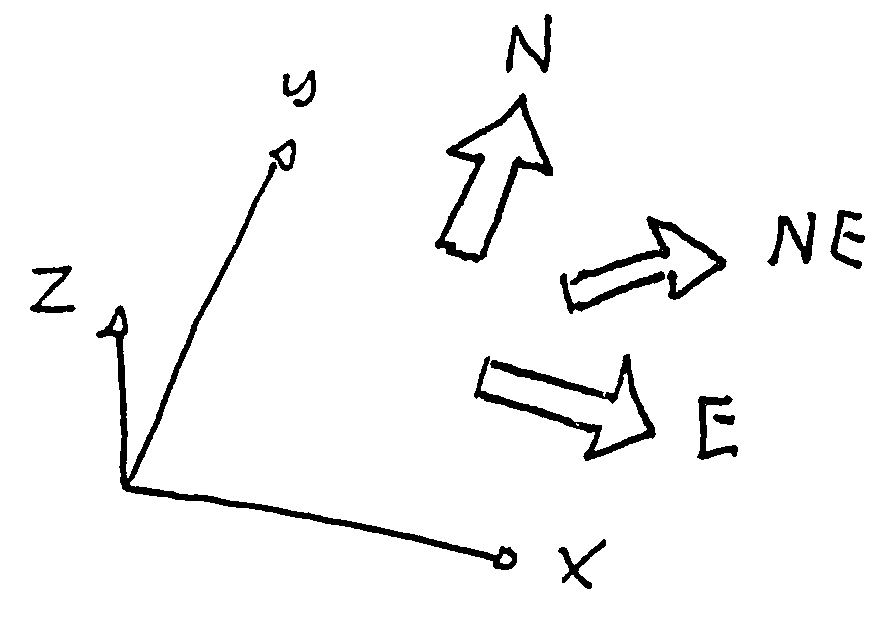
\includegraphics[height=3.5cm]{2021-1-C3/20210813_direcoes.pdf}
$$

\newpage

{\bf Exercício 7 (cont.)}

\ssk

d) Desenhe a trajetória associada a $α=0$, $β=-1$

e diga o nome da direção dela.

\ssk

e) Desenhe a trajetória associada a $α=-1$, $β=1$.

e diga o nome da direção dela.

\ssk

f) Quais são os valores mais simples de $α$ e $β$ ---

onde ``simples'' quer dizer ``$0$, $1$ ou $-1$'' --- que fazem

a trajetória ir pro nordeste? E pro sudoeste?

\bsk
\bsk

Nos próximos exercícios eu vou me referir a essas

trajetórias em que $α$ e $β$ são números ``simples''

pelos \ColorRed{nomes das direções} delas.


\newpage

% «zt-e-ztt-intro»  (to ".zt-e-ztt-intro")
% (c3m211qp 13 "zt-e-ztt-intro")
% (c3m211qa    "zt-e-ztt-intro")

{\bf O significado geométrico de $z_t$}

Nós sabemos calcular $z$, $z_t$ e $z_{tt}$ a partir de $t$,

e sabemos calcular $z$, $z_t$ e $z_{tt}$ em $t_0$.

\ssk

Com um pouquinho de esforço você deve ser

capaz de visualizar o que acontece perto de $t_0$...

o valor da primeira derivada, $(z_t)(t_0)$, diz o seguinte:

\def\LR{$\Longleftrightarrow$}

\msk

\begin{tabular}{lll}
$z$ aumenta quando $t$ aumenta (``crescente'')   &\LR& $(z_t)(t_0)>0$ \\
$z$ ``fica horizontal'' quando $t$ aumenta       &\LR& $(z_t)(t_0)=0$ \\
$z$ diminui quando $t$ aumenta (``decrescente'') &\LR& $(z_t)(t_0)<0$ \\
\end{tabular}

\bsk
\bsk

\ColorRed{

Veja o vídeo!!!

}

\ssk

{\footnotesize

% (c3m211qa "video-3")

\url{http://angg.twu.net/eev-videos/2021-1-C3-funcoes-quadraticas-3.mp4}

\url{https://www.youtube.com/watch?v=VwowES6EM3Y}

}

\newpage

% «signif-geom-ztt»  (to ".signif-geom-ztt")
% (c3m212dnp 19 "signif-geom-ztt")
% (c3m212dna    "signif-geom-ztt")

{\bf O significado geométrico de $z_{tt}$}

Nos casos em que $z$ ``fica horizontal'' nós vamos usar

a segunda derivada, $(z_{tt})(t_0)$, pra ver se o gráfico de

$z(t)$ ``parece uma parábola'' ao redor de $t_0$, e se essa

parábola tem concavidade pra cima ou pra baixo:

\msk

\begin{tabular}{lll}
concavidade pra cima  &\LR& $(z_{tt})(t_0)>0$ \\
``parece horizontal'' &\LR& $(z_{tt})(t_0)=0$ \\
concavidade pra baixo &\LR& $(z_{tt})(t_0)<0$ \\
\end{tabular}

\bsk

Eu usei muitos termos informais de propósito.

No \ColorRed{próximo exercício} você vai tentar descobrir

\ColorRed{sem fazer contas} qual é o comportamento da $z$

em torno de $t_0$, e no \ColorRed{outro exercício} você vai

\ColorRed{fazer as contas} e vai ver se o seu olhômetro

funcionou direito.


\newpage

% «exercicio-8»  (to ".exercicio-8")
% (c3m212dnp 20 "exercicio-8")
% (c3m212dna    "exercicio-8")
% (c3m211qp 15 "exercicio-5")
% (c3m211qa    "exercicio-5")

{\bf Exercício 8.}

\unitlength=20pt


Em cada um dos desenhos dos próximos slides diga

o que acontece quando a trajetória $(x(t),y(t))$ anda

em uma das oito direções simples, que são:

\msk

norte, nordeste, leste, sudeste,

sul, sudoeste, oeste, noroeste.

\bsk

Use estas categorias na suas respostas:

\msk

$z$ cresce

$z$ decresce

$z$ faz uma parábola com concavidade pra cima

$z$ faz uma parábola com concavidade pra baixo

$z$ é ``muito horizontal''




%L qf = QuadraticFunction {x0=3, y0=2, a=2, Dx=0, Dy=0, Dxx=1, Dyy=1, Dxy=0}
%L srf = Surface.new(qf, 3, 2)
\pu
$$\QuadraticInPerspective{srf}
$$



\newpage

%L qf = QuadraticFunction {x0=3, y0=2, a=2, Dx=0, Dy=0, Dxx=1, Dyy=-1, Dxy=0}
%L srf = Surface.new(qf, 3, 2)
\pu
$$\QuadraticInPerspective{srf}
$$








\newpage

% (c3m211cna "video-1")
% (c3m211cna "video-2")

% (c3m212dnp 3 "links")
% (c3m212dna   "links")


% (c3m211cnp 2 "links")
% (c3m211cna   "links")

PDFs antigos:

\msk

Sobre ``adivinhar trajetórias'':

{\footnotesize

% (c3m211vtp 6 "sobre-adivinhar-trajetorias")
% (c3m211vta   "sobre-adivinhar-trajetorias")
% http://angg.twu.net/LATEX/2021-1-C3-vetor-tangente.pdf#page=6
\url{http://angg.twu.net/LATEX/2021-1-C3-vetor-tangente.pdf\#page=6}

}

\msk

Diagramas de numerozinhos (2020.2):

{\footnotesize

% (c3m202rcadeia1p 14 "exercicio-6")
% (c3m202rcadeia1a    "exercicio-6")
% http://angg.twu.net/LATEX/2020-2-C3-rcadeia1.pdf#page=14
\url{http://angg.twu.net/LATEX/2020-2-C3-rcadeia1.pdf\#page=14}

}

\msk

Mini-teste sobre cortes em superfícies no olhômetro (2020.2):

{\footnotesize

% (c3m202mt1p 4 "figura-intro")
% (c3m202mt1a   "figura-intro")
% http://angg.twu.net/LATEX/2020-2-C3-MT1.pdf#page=4
\url{http://angg.twu.net/LATEX/2020-2-C3-MT1.pdf\#page=4}

}


\msk

Questão 1 da P1 de 2020.2:

{\footnotesize

% (c3m202p1p 8 "gabarito-1")
% (c3m202p1a   "gabarito-1")
% http://angg.twu.net/LATEX/2020-2-C3-P1.pdf#page=8
\url{http://angg.twu.net/LATEX/2020-2-C3-P1.pdf\#page=8}

}

\msk

Curvas de nível e diagramas de numerozinhos (2021.1):

\ssk

{\footnotesize

% (c3m211cnp 3 "exercicio-1")
% (c3m211cna   "exercicio-1")
%    http://angg.twu.net/LATEX/2021-1-C3-curvas-de-nivel.pdf#page=3
\url{http://angg.twu.net/LATEX/2021-1-C3-curvas-de-nivel.pdf#page=3}

}

\ssk





\newpage


%\printbibliography

\GenericWarning{Success:}{Success!!!}  % Used by `M-x cv'

\end{document}

%  ____  _             _         
% |  _ \(_)_   ___   _(_)_______ 
% | | | | \ \ / / | | | |_  / _ \
% | |_| | |\ V /| |_| | |/ /  __/
% |____// | \_/  \__,_|_/___\___|
%     |__/                       
%
% «djvuize»  (to ".djvuize")
% (find-LATEXgrep "grep --color -nH --null -e djvuize 2020-1*.tex")

 (eepitch-shell)
 (eepitch-kill)
 (eepitch-shell)
# (find-fline "~/2021.2-C3/")
# (find-fline "~/LATEX/2021-2-C3/")
# (find-fline "~/bin/djvuize")

cd /tmp/
for i in *.jpg; do echo f $(basename $i .jpg); done

f () { rm -v $1.pdf;  textcleaner -f 50 -o  5 $1.jpg $1.png; djvuize $1.pdf; xpdf $1.pdf }
f () { rm -v $1.pdf;  textcleaner -f 50 -o 10 $1.jpg $1.png; djvuize $1.pdf; xpdf $1.pdf }
f () { rm -v $1.pdf;  textcleaner -f 50 -o 20 $1.jpg $1.png; djvuize $1.pdf; xpdf $1.pdf }

f () { rm -fv $1.png $1.pdf; djvuize $1.pdf }
f () { rm -fv $1.png $1.pdf; djvuize WHITEBOARDOPTS="-m 1.0 -f 15" $1.pdf; xpdf $1.pdf }
f () { rm -fv $1.png $1.pdf; djvuize WHITEBOARDOPTS="-m 1.0 -f 30" $1.pdf; xpdf $1.pdf }
f () { rm -fv $1.png $1.pdf; djvuize WHITEBOARDOPTS="-m 1.0 -f 45" $1.pdf; xpdf $1.pdf }
f () { rm -fv $1.png $1.pdf; djvuize WHITEBOARDOPTS="-m 0.5" $1.pdf; xpdf $1.pdf }
f () { rm -fv $1.png $1.pdf; djvuize WHITEBOARDOPTS="-m 0.25" $1.pdf; xpdf $1.pdf }
f () { cp -fv $1.png $1.pdf       ~/2021.2-C3/
       cp -fv        $1.pdf ~/LATEX/2021-2-C3/
       cat <<%%%
% (find-latexscan-links "C3" "$1")
%%%
}

f 20201213_area_em_funcao_de_theta
f 20201213_area_em_funcao_de_x
f 20201213_area_fatias_pizza



%  __  __       _        
% |  \/  | __ _| | _____ 
% | |\/| |/ _` | |/ / _ \
% | |  | | (_| |   <  __/
% |_|  |_|\__,_|_|\_\___|
%                        
% <make>

 (eepitch-shell)
 (eepitch-kill)
 (eepitch-shell)
# (find-LATEXfile "2019planar-has-1.mk")
make -f 2019.mk STEM=2021-2-C3-diag-nums veryclean
make -f 2019.mk STEM=2021-2-C3-diag-nums pdf

% Local Variables:
% coding: utf-8-unix
% ee-tla: "c3dn"
% ee-tla: "c3m212dn"
% End:
